\documentclass{article}
\usepackage[english]{babel}
\usepackage[utf8]{inputenc}
\usepackage{fancyhdr}
\usepackage{tabularx}
\usepackage{graphicx}
\usepackage{amsfonts}
\usepackage{multicol}
\pagestyle{fancy}
\fancyhf{}
\rhead{Page \thepage}
\lhead{Team Number: 15559}
\cfoot{\thepage}

\begin{document}
% TITLE
\begin{center}
\textbf{\huge Remote Work: \textit{Fad or Future}}
\end{center}

\setcounter{section}{-1}

% Executive Summary
\section{Executive Summary}
\indent
When the COVID-19 pandemic disrupted every avenue of life, millions of working individuals adjusted through telecommuting. Now, the question is whether remote work will remain a part of the new normal. Our team’s goal is to model the trajectory of remote work in select cities for 2024 and 2027, considering pertinent factors such as the availability of remote-ready jobs, employer decisions, and employee choices.

\indent
To begin, we calculated the maximum number of individuals in a city who could feasibly work remotely in their current job position. In other words, we wanted to find the “remote-ready” work population for each city. To do so, we multiplied the percentage of individuals in each industry that could work from home by the predicted number of individuals in a given industry over the period 2022-2027. To predict the latter value, we performed linear regression on the provided M3 Mathworks data for the number of individuals in each industry in each city over time. We thus predicted remote-ready population for each city for the years 2024 and 2027. Despite having some low R2 values, the year was sometimes a poor predictor of the number of individuals  in an industry, the model that combined numerous linear regressions yielded reasonable results for the remote-ready populations for the years 2024 and 2027.

\indent
Furthermore, to predict whether an individual worker will choose to work remotely full-time and gain employer approval, we created a random forest classification based on relevant factors to the employee choice such as age, gender, and parental status. This yielded a relatively good accuracy of 0.74, and we identified age as the most important factor in the worker’s decision to work remotely or in person. We  accounted for the employer’s likelihood to allow the employee to work remotely with a random probability generation.

\indent
	Finally, to use our model that predicted whether both the employer and a given individual would both agree to work remotely for the five cities, we simulated 5000 citizens of each city. The simulation accounted for the unique distribution of ages, genders, and children for each city and provided us with the percent of employees and employers that would agree on fully remote working plans, given that the individual’s job could be completed remotely. Combining these 5 percentages for employee and employer cooperation, we have found predictions for all 3 years for all 5 cities for the number of individuals that will work remotely. We have found that Barry will see the greatest impact from remote work by the year 2024, and Seattle by 2027.

\indent
	Although the long-term ramifications of the COVID-19 pandemic on the workplace are still in limbo, modeling is nonetheless a powerful tool to make useful predictions. As the world settles upon a new normal, we believe that continuing to collect data and improving upon previous models will ultimately allow us to keep modeling the future.



\newpage
\tableofcontents
\newpage

\noindent
\textbf{\large Global Definitions}
\begin{itemize}
    \item We define a remote-ready job as a position where an employee can satisfactorily complete the position objectives without doing so from a workplace.
\end{itemize}
\noindent
\textbf{\large Global Assumptions}
\begin{enumerate}
    \item \textit{There will be no significant policy changes regarding standards for remote work in the next 5 years.} Due to the unpredictability of new legislation, we cannot account for these changes.
    \item \textit{In accordance with our definition of “remote-ready”, partially remote jobs do not qualify as remote-ready.} The complete lack of time in the workplace is inherent to being completely remote and thus “remote-ready”.
    \item \textit{An adult is defined across both the US and the UK as a person 18 years of age or older, and a child is defined as below 18 years of age.} In order to differentiate between adults and children when analyzing census data, the distinction is imperative for simplicity’s sake.
\end{enumerate}

\section{Part I: Ready or Not}
\

\subsection{Restatement of the Problem}
% Restate the problem here
We are tasked with creating a model to estimate the percentage of jobs currently ready for remote work and then use said model to predict the percentage of remote-ready jobs in 2024 and 2027. We will apply this model to the following cities:
\begin{itemize}
    \item Seattle, WA, US
    \item Omaha, NE, US
    \item Scranton, PA, US
    \item Liverpool, England, UK
    \item Barry, Wales, UK
\end{itemize}

\

\subsection{Assumptions}
% Add all assumptions
\begin{enumerate}
    \item \textit{In accordance with our definition of “remote-ready”, partially remote jobs do not qualify as remote-ready.} The complete lack of time in the workplace is inherent to being completely remote and thus “remote-ready”.
    
    \item \textit{COVID-19 developments during or after 2023 will not affect a worker’s status as remote-ready or not remote-ready.} Modeling by Emory University \cite{news_2021} and experts \cite{spencekimball_2022} predict that COVID will be endemic (“circulating in the general population”) in the US and UK by 2023. Accordingly, new COVID-19 variants and infection spikes will not change a worker’s status as remote or in-person.
    
    \item \textit{Public sentiment towards working remotely will not significantly change from the present.} Although firms may attempt to influence the public’s perception of working remotely, the evidence regarding similar or greater productivity levels of remote workers compared to in-person workers \cite{wfh} and the favorable anecdotal experiences of a large portion of the population regarding remote work during the COVID pandemic period \cite{owllabs} (2020-2022) will keep the public’s perception of remote work as moderately favorable.
    
    \item \textit{We do not account for automation’s future impact on the sector makeup of the labor force.} Automation varies significantly based on the urban versus rural characteristics of cities and towns. For example, Seattle, WA, a high-growth hub according to the McKinsey Institute, will be automated in 2027 to a higher degree than Scranton, PA, in the “mixed middle” of economic growth.\cite{mckinsey} Additionally, the McKinsey Institute indicates that the bulk of automation will manifest on a 10-15 year timeline, rather than the 5-year timeline to 2027.

\end{enumerate}
\

\subsection{Variables Used} \indent
\begin{table}[h]
\centering
\begin{tabularx}{\linewidth}{|l|>{\raggedright\arraybackslash}X|>{\raggedright\arraybackslash}X|}
\hline
    \textbf{Symbol} & \textbf{Definition} & \textbf{Units} \\
    \hline
    $\hat{P_i}$ & Predicted number of people in industry \textit{i} in a given year & People   \\
    \hline
    $\mu_i$ & Percentage of individuals in industry \textit{i} that can work from home & \dots \\
    \hline
    $RR_c$ & Number of individuals in city \textit{c} that are remote-ready & People \\
    \hline
\end{tabularx}
\end{table}

\

\subsection{Model Development}
% Write about model development
For any city, the number of individuals that are remote-ready is given by 
\[
RR_c = \sum \hat{P_i} \cdot \mu_i,
\]
\indent
Where $\hat{P_i}$ is the predicted number of individuals in industry \textit{i} in city \textit{c} in a given year, and $\mu_i$ is the percentage of those individuals that are remote-ready. \\
In order to predict the number of individuals in any city that are remote-ready, we must first take into account how many individuals are employed in each industry for that city during a given year, $\hat{P_i}$, since each industry has its own characteristics and responses to remote work pressures. In order to do this, we performed linear regression on the D1 city employment data provided by the 2022 MathWorks Math Modeling Challenge \cite{m3data}. The number of individuals employed in each industry for each given city is the response variable, while the year, ranging from 2000 to 2021, is the explanatory variable.

The reason we chose linear regression was simply because of the large number of regression analyses needed to be computed. It is impractical to analyze each industry for each city, and decide whether it follows an exponential, polynomial, or any pattern. Therefore, linear regression was employed because it offers a simple, consistent measure of predicting industry growth or decline in any given city. \\

It is worth noting that UK cities did not have data for the year 2000. \\
The results of each linear regression are as follows: \\
\begin{table}[h]
\centering
\textbf{Seattle} \\
\begin{tabularx}{210pt}{|c|X|c|X|c|X|}
    \hline
    \textbf{Industry} & \textbf{2024} & \textbf{2027} \\
    \hline
    Mining, logging, constr. & 122281 & 125811 \\
    \hline
    Manufacturing & 157608 & 152571 \\
    \hline
    Trade, transp., and util. & 378727 & 387780 \\
    \hline
    Information & 140115 & 149243  \\
    \hline
    Financial Activities & 93710 & 92559 \\
    \hline
    Professional and Bus. & 303718 & 316277 \\
    \hline
    Education and Health & 275938 & 287018 \\
    \hline
    Leisure and Hospit. & 170387 & 172776 \\
    \hline
    Other Services & 72090 & 73726 \\
    \hline
    Government & 255364 & 256008\\
    \hline
\end{tabularx}
\end{table}
\begin{table}[h]
\centering
\textbf{Omaha} \\
\begin{tabularx}{210pt}{|c|X|c|X|c|X|}
    \hline
    \textbf{Industry} & \textbf{2024} & \textbf{2027} \\
    \hline
    Mining, logging, constr. & 30905 & 32015 \\
    \hline
    Manufacturing & 32617 & 32452 \\
    \hline
    Trade, transp., and util. & 91253 & 89586 \\
    \hline
    Information & 9023 & 8314  \\
    \hline
    Financial Activities & 46911 & 48322 \\
    \hline
    Professional and Bus. & 75092 & 77036 \\
    \hline
    Education and Health & 84683 & 88202 \\
    \hline
    Leisure and Hospit. & 49255 & 50274 \\
    \hline
    Other Services & 19165 & 19652 \\
    \hline
    Government & 68482 & 69854 \\
    \hline
\end{tabularx}
\end{table}
\newpage
\begin{table}[h]
\centering
\textbf{Scranton} \\
\begin{tabularx}{210pt}{|c|X|c|X|c|X|}
    \hline
    \textbf{Industry} & \textbf{2024} & \textbf{2027} \\
    \hline
    Mining, logging, constr. & 10003 & 9946 \\
    \hline
    Manufacturing & 22881 & 20657 \\
    \hline
    Trade, transp., and util. & 64761 & 65854 \\
    \hline
    Information & 1730 & 1050  \\
    \hline
    Financial Activities & 12727 & 12646 \\
    \hline
    Professional and Bus. & 28168 & 28786 \\
    \hline
    Education and Health & 53975 & 54826 \\
    \hline
    Leisure and Hospit. & 20523 & 20449 \\
    \hline
    Other Services & 7492 & 7170 \\
    \hline
    Government & 27913 & 27382 \\
    \hline
\end{tabularx}
\end{table}

\begin{table}[h]
\centering
\textbf{Liverpool} \\
\begin{tabularx}{210pt}{|c|X|c|X|c|X|}
    \hline
    \textbf{Industry} & \textbf{2024} & \textbf{2027} \\
    \hline
    Mining, logging, constr. & 150979 & 153097 \\
    \hline
    Manufacturing & 108080 & 113806 \\
    \hline
    Trade, transp., and util. & 160456 & 171263 \\
    \hline
    Information & 75737 & 78003  \\
    \hline
    Financial Activities & 23212 & 23451 \\
    \hline
    Professional and Bus. & 43108 & 43553 \\
    \hline
    Education and Health & 21309 & 20326 \\
    \hline
    Leisure and Hospit. & 67673 & 68047 \\
    \hline
    Other Services & 76853 & 77403 \\
    \hline
    Government & 22463 & 21717 \\
    \hline
\end{tabularx}
\end{table}
\newpage
\begin{table}[h]
\centering
\textbf{Barry} \\
\begin{tabularx}{210pt}{|c|X|c|X|c|X|}
    \hline
    \textbf{Industry} & \textbf{2024} & \textbf{2027} \\
    \hline
    Mining, logging, constr. & 4061 & 4076 \\
    \hline
    Manufacturing & 4785 & 4775 \\
    \hline
    Trade, transp., and util. & 1143 & 1130 \\
    \hline
    Information & 3754 & 3689  \\
    \hline
    Financial Activities & 3740 & 3855 \\
    \hline
    Professional and Bus. & 6945 & 7158 \\
    \hline
    Education and Health & 10953 & 11151 \\
    \hline
    Leisure and Hospit. & 10333 & 10333 \\
    \hline
    Other Services & 3098 & 3108 \\
    \hline
    Government & 10953 & 11151 \\
    \hline
\end{tabularx}
\end{table}

\begin{table}[ht]
\centering
\begin{tabularx}{\linewidth}{|c|X|c|X|c|X|c|X|c|X|}
\hline
    $R^2$ Values & Seattle & Omaha & Scranton & Liverpool & Barry \\
    \hline
    Mining, logging, constr. & 0.364 & 0.601 & 0.108 & 0.49 & 0.004 \\
    \hline
    Manufacturing & 0.387 & 0.109 & 0.745 & 0.719 & 0.001 \\
    \hline
    Trade, transp., and util. & 0.429 & 0.695 & 0.917 & 0.987 & 0.011 \\
    \hline
    Information & 0.856 & 0.917 & 0.991 & 0.867 & 0.27 \\
    \hline
    Financial Activities & 0.228 & 0.949 & 0.246 & 0.074 & 0.279 \\
    \hline
    Professional and Bus. & 0.809 & 0.835 & 0.458 & 0.074 & 0.279 \\
    \hline
    Education and Health & 0.668 & 0.956 & 0.565 & 0.667 & 0.307 \\
    \hline
    Leisure and Hospit. & 0.063 & 0.491 & 0.007 & 0.038 & 0 \\
    \hline
    Other Services & 0.343 & 0.782 & 0.752 & 0.102 & 0.001 \\
    \hline
    Government & 0.005 & 0.776 & 0.784 & 0.342 & 0.307 \\
    \hline
\end{tabularx}
\end{table}
While some $r^2$ values and correlation coefficients are exceptionally low, these low correlations for an industry versus year effectively means that predicted values for $\hat{P_i}$ will be close to the calculated average value of the 5-6 data points analyzed by the linear model. That is an outcome that remains reasonable, and the $\hat{P_i}$ predictions of our linear regression models with $r^2$ values close to zero, should not be discounted. 

Since each industry’s work is remarkably different and certain industries are more capable of transitioning to remote work than others, the percent of individuals employed in each industry that can work remotely must be quantified and taken into account by the model. \\
\indent The Remote Work data provided by the 2022 MathWorks Math Modeling Challenge contains this information, broken down into different industries than the industries listed in D1 industry employment data. Therefore, the following re-categorizations have been made,
\newpage
\begin{table}[h]
\centering
\begin{tabularx}{\linewidth}{|l|>{\raggedright\arraybackslash}X|}
\hline
    \textbf{D1} & \textbf{D3 change these headers} \\ \hline
    Mining, logging, construction & Farming, fishing and forestry; Installation, maintenance and repair; Construction and extraction; Building and grounds cleaning and maintenance \\ \hline
    Manufacturing & Production \\ \hline
    Trade, transportation, and utilities & Transportation and material moving \\ \hline
    Information & Computer and mathematical; Legal; Life, physical and social science; Architecture and engineering \\ \hline
    Financial activities & Business and financial operations; Sales and related \\ \hline
    Professional and business services & Management; Office and administrative \\ \hline
    Education and Health Services & Education, training and library; Healthcare practitioners and technical; Healthcare support \\ \hline
    Leisure and hospitality & Arts, design, entertainment, sports and media; Personal care and service \\ \hline
    Other services & Community and social service \\ \hline
    Government & Protective service \\ \hline
\end{tabularx}
\end{table}

After averaging the estimated percentage of jobs that can be done at home by occupation category given by D3 for each industry category given by D1, we obtain the following values of $\mu_i$ for each industry:
\newpage
\begin{table}[ht]
\centering
\begin{tabularx}{210pt}{|c|X|c|X|}
\hline
    \textbf{Industry} &  $\mathbf{\mu_i}$ \\ \hline
    Mining, logging, construction & 0.50\% \\ \hline
    Manufacturing & 1.00\% \\ \hline
    Trade, transportation, and utilities & 3.00\% \\ \hline
    Information & 78.00\% \\ \hline
    Financial activities & 58.00\% \\ \hline
    Professional and business services & 76.00\% \\ \hline
    Education and Health Services & 35.00\% \\ \hline
    Leisure and hospitality & 51.00\% \\ \hline
    Other services & 37.00\% \\ \hline
    Government & 6.00\% \\ \hline
\end{tabularx}
\end{table}

Then, the $RR_c$ for each city can be calculated as a function of year with the equation
\[
    RR_c = \sum \hat{P_i} \cdot \mu_i,
\]
and the results are displayed in the following graphs:
% insert graphs
\

\subsection{Results}
% Write about results of the model
Using the population of each industry, $\hat{P_i}$, that we found in the first portion and the percentages of jobs that are remote-ready by each industry, $\mu_i$, we can then calculate the percentage of remote ready jobs in 2024 and 2027 using our formula. This gives us the following results:
\begin{table}[h]
\centering
\begin{tabularx}{\linewidth}{|l|>{\raggedright\arraybackslash}X|>{\raggedright\arraybackslash}X|}
\hline
    \textbf{City} & \textbf{Predicted Percentage of remote-ready jobs in 2024} & \textbf{Predicted Percentage of remote-ready jobs in 2027} \\
    \hline
    Seattle & 32.16\% & 32.55\%   \\
    \hline
    Omaha & 31.63\% & 31.84\% \\
    \hline
    Scranton & 26.45\% & 26.60\% \\
    \hline
    Liverpool & 24.50\% & 24.18\% \\
    \hline
    Barry & 35.78\% & 35.82\% \\
    \hline
\end{tabularx}
\end{table}
\indent
These results are reasonable, proving that even though some $r^2$ values of the linear regression models had low $r^2$ values, the combination of all the different linear regression models yields a robust prediction for the Predicted Percentage for remote-ready in 2024. For example, the decrease predicted percentage of remote-ready in Liverpool makes sense, since it is the only city that had a large increase in employment in the manufacturing industry over the years 2005-2021.
\indent
Furthermore, we can compare this predicted remote-ready data for 2021 with the provided M3 Mathworks data in sheet D4. Seeing that in the months from March 2020 to September 2021, the percentage of US workers who worked from home exclusively had a maximum value of 54\%, but quickly corrected to around 35-25\%, we can infer that our predicted percentage remote-ready for the US served as a sustainable percentage.

\begin{figure}
  \centering
  \includegraphics[width=.45\linewidth]{seattle.png}
  \caption{Seattle.}
  \label{fig:SeattleQ1}
\end{figure}
\begin{figure}
  \centering
  \includegraphics[width=.45\linewidth]{scranton.png}
  \caption{Scranton.}
  \label{fig:ScrantonQ1}
\end{figure}

\begin{figure}
  \centering
  \includegraphics[width=.45\linewidth]{OMaha.png}
  \caption{Omaha.}
  \label{fig:OmahaQ1}
\end{figure}
\newpage
\begin{figure}
  \centering
  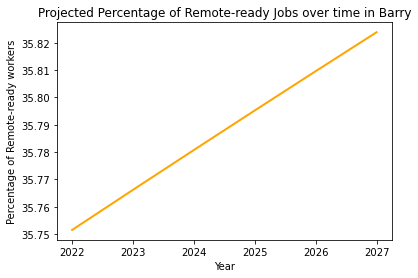
\includegraphics[width=.55\linewidth]{Barry.png}
  \caption{Barry.}
  \label{fig:BarryQ1}
\end{figure}

\begin{figure}
  \centering
  \includegraphics[width=.55\linewidth]{Liverpool.png}
  \caption{Liverpool.}
  \label{fig:LiverpoolQ1}
\end{figure}

\newpage
\
\subsection{Strengths and Weaknesses}

% Write about strengths and weaknesses
\indent
A major challenge when considering the COVID-19 pandemic is its inherently volatile and unpredictable nature. It would be extremely difficult to account for all the possible scenarios, so it was necessary for us to make a simplification to create a useful model. Barring a major change like the emergence of a new variant, current models predict a trajectory in which the disease will become endemic to the United States and United Kingdom by 2023. Assuming a constant endemic state for COVID-19 allows our model to not be affected by drastic changes in the disease’s epidemiology between 2024 and 2027.

From the $r^2$ table, we can see a wide range of $r^2$ values. For example, most of the variability in the information industry employment in Scranton can be accounted for by the change in year ($r^2$ = 0.991). On the other hand, very little variation seen in the leisure and hospitality industry in Liverpool can be explained by the change in year ($r^2$ = 0.007). The extremely small data set contributes to this wide variability in the $r^2$ values. Our models could be improved by adding more data points, which would increase both the $r$ and $r^2$ values to improve their prediction capabilities.


\section{Part II: Remote Control}
\

\subsection{Restatement of the Problem}
% Restate the problem here
In this problem, we are tasked with creating a model to predict whether an individual worker with a remote-ready job will be allowed to and will choose to work from home.
\

\subsection{Assumptions}
% Add all assumptions
\begin{enumerate}
    \item \textit{When considering an individual worker whose job is remote-ready, we assume that the probability that they are allowed to work from home by their employer and their desire to work from home are independent.} This allows us to individually consider each of these likelihoods and then find the product of them to calculate the probability of both events occurring. Additionally, Forbes reports a sizable disconnect between the groups on returning to the office \cite{segal_2021}.
    \item \textit{Employer sentiment towards remote work in 2021 will remain roughly constant until 2027.} While we understand that employer sentiment may vary by 2027, data on employer sentiment is only available up until the present. Additionally, we make the global assumption that COVID-19 will be endemic by 2024, so employer sentiment should not be largely affected by COVID-19 past that point.
    \item \textit{Only age, gender, and the presence of children in the household affect a worker’s decision to work remotely.}  This is the information our data included. Analysis from the Bureau of Labor Statistics supports that these are very important factors in the decision to work from home \cite{usbls}.
    \item \textit{All employers are equally likely to deny or allow fully remote work.} Data on variations by industry was scarce, and this assumption allowed us to focus on the random forest.
\end{enumerate}
\

\subsection{Variables Used} 
\indent
Age is an incredibly relevant factor in the decision to work remotely or in the workplace. The older members of the workforce may feel more comfortable with face-to-face interaction, whereas younger generations consider virtual interactions as commonplace and convenient. The Hartford reports 50\% of small business owners ages 18-34 say remote workers are more productive than office workers, whereas only 15\% of small business owners over 65 find remote workers more productive than in-person employees\cite{spors_2020}.
\indent
Gender is another indicator of the remote versus in-person work decision. A Flexjobs survey indicates 68\% of women prefer to work remotely post-pandemic compared to only 57\% of men. 80\% of women consider it a key job benefit, whereas only 69\% of men thought the same\cite{pelta_2022}. This may be due to the higher proportion of housework that women do; the 2020 Women in the Workplace report found mothers were 1.5 times more likely than fathers to spend an extra three or more hours per day on housework\cite{lean_in}. Remote work is a method of balancing these requirements. 
\indent
This leads into another factor to consider: parenthood. The additional duties of childcare can make remote work a helpful option to parents. Another Flexjobs survey found 61\% of parents want to stay remote full-time, with 62\% saying they would quit their current job if they cannot continue remotely\cite{flexjobs_2022}.
\indent
On the other side of the decision to work remotely or in-person is the employer. As employees demand flexibility in work hours and arrangements, Owl Labs found 26\% of employers are allowing employees to work remotely full-time \cite{owllabs}. We rounded this to 25\% for ease.
\
\subsection{Model Development}
% Write about model development
\indent
We employed the Scikit-learn library in Python to train a random forest classifier model on the factors described above. Random forest classifiers employ decision trees trained on random samples of the data set to isolate variables and average the predictions of each tree, resulting in a robust prediction. 

Our model is trained on the results of a random survey sourced from Kaggle regarding professionals’ demographics and their decision to stay remote or return to the workplace \cite{kaggle}. Our target was the column ‘Same\_office\_home\_location’ (renamed to ‘WFH’), or if the professional’s workplace was in the home. After splitting the data set into training and test sets, our model used 100 trees with a maximum depth of five nodes to make predictions regarding if a given professional would choose to work from home. \\
\indent
To account for the approximate one-fourth of employers who are allowing employees to work from home full-time, we randomly generated a number from 1-4 inclusive using the random Python library in each instance that an employee’s classification in the random forest was to work virtually. If the randomly generated number was 1, then the request was approved. This aligns with the approximate 25\% of employers who are allowing fully remote work.

\


\subsection{Results}
% Write about results of the model
\indent
The Random forest regression reached an \textbf{accuracy classification score of 0.74}. This is an acceptable accuracy given the time and data constraints present. We were additionally able to analyze the importance of the respective features using the feature\_importances\_ variable from the random forest algorithm in scikit-learn.

\indent
We ultimately determined age is the most important feature with an importance of .75 in the classification model, followed by gender at .13 importance and then children at .12 importance. 
\begin{figure}
  \centering
  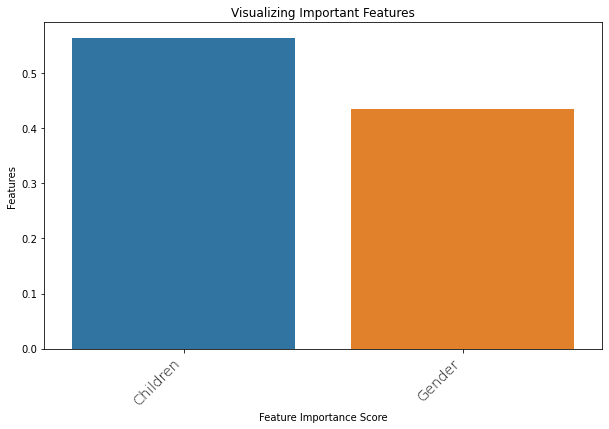
\includegraphics[width=.55\linewidth]{import.png}
  \caption{Important Features of Random Forest Classification.}
  \label{fig:ImportantQ2}
\end{figure}
\

\subsection{Strengths and Weaknesses}
% Write about strengths and weaknesses
\indent
With a small data set of 207 respondents, the random forest classification’s ability to mitigate the individual over fitting of decision trees with the averaging of a large number of decision trees is advantageous. This yielded a higher predictive accuracy than a single decision tree by itself. 

\indent
Additionally, the random tree forest allows us to effectively combine features and identify the important features in the classification. We were able to determine that age is most closely linked to the employee decision to work remotely or in-person. However, this does bring us to a limitation of our data set, as we were not able to account for other factors likely to have an impact, such as education or income, because the data set did not include them. To improve upon this model, we would find a suitable data set with the factors of income and education and retrain the random forest. A specific shortcoming of the random forest model is the difficulty to ascertain the exact decision trees because of the large quantity of decision trees. We would also like to incorporate another random forest for the employer’s choice, based on industry, company size, etc. given more time.

\

\section{Part III: Just a Little Home-work}
\

\subsection{Restatement of the Problem}
% Restate the problem here
In this problem, we are tasked with creating a model that predicts whether an individual worker whose job is remote-ready will be allowed to and will choose to work from home.
\

\subsection{Assumptions}
% Add all assumptions
\begin{enumerate}
    \item \textit{The working adult population is aged 20-65.} 62 years old is the average retirement age, so 65 is a reasonable upper cutoff\cite{loriekonish_2022}. Additionally, setting the lower cutoff at the age of 20 years allows for an easier analysis of census data, which groups ages by 5 years per stratum. Since these age bounds encapsulate the vast majority of working individuals, it was sufficient for our model. 
    \item \textit{The demographics of the working adult population are consistent with the demographics of the general adult population of a given city.} This allows us to utilize census data, which is more readily available for the general adult population than the working adult population.
    \item \textit{An individual’s employment in a given industry is independent of their age, number of children, or gender.} While this is unlikely to be true, it allows us to conduct a simulation that determines the proportion of the remote-ready population that will actually work from home.
    \item \textit{The proportion of households with children that have 2 adults and the proportion of households with children that have 1 adult is consistent across the US and the UK.} If a household with children does not have 2 adults, we assume it has 1 adult. This allows us to find the average number of adults in a household with children.
    \item \textit{The age, gender, and child status data will not change over time.}

\end{enumerate}
\

\subsection{Variables Used}
\begin{table}[h]
\centering
\begin{tabularx}{\linewidth}{|l|>{\raggedright\arraybackslash}X|>{\raggedright\arraybackslash}X|}
\hline
    \textbf{Symbol} & \textbf{Definition} & \textbf{Units} \\
    \hline
    $K_c$ & Proportion of adult population in city \textit{c} that has kids. & \dots   \\
    \hline
    $HC_c$ & Number of households in city \textit{c} with children. & Households \\
    \hline
    $F_c$ & Proportion of adult population of city \textit{c} that is female. & \dots \\
    \hline
    $P_c$ & Adult population of city \textit{c}. & People \\
    \hline
    $A_c(Age_a-Age_b)$ & Proportion of total adult population that has age between $Age_a$ and $Age_b$ for city \textit{c}. & \dots \\ \hline
\end{tabularx}
\end{table}

\

\subsection{Model Development}
The proportion of adults within a city with children $A_c$, is given by
\[
K_c = \frac{HC_c \cdot 0.69 \cdot 2 + HC_c \cdot 0.31}{P_c},
\]

Since a household that has children (people under 18), there is a probability of 69\% that there are two parents in the household \cite{bureau_2021}. Since we have assumed that the remaining 31\% of households with children have only one parent in them, the above equation yields the proportion of the adult population in a given city c that has children.

We used US census and UK census data to find the number of households in each city that have children ($HC_c$), performed the necessary calculations, and have summarized the data in the following table
\begin{table}[ht]
\centering
\begin{tabularx}{37mm}{|c|X|c|X|}
\hline
    $K_{Seattle}$ & 16.27\% \\ \hline
    $K_{Omaha}$ & 25.13\% \\ \hline
    $K_{Scranton}$ & 22.66\% \\ \hline
    $K_{Liverpool}$ & 21.54\% \\ \hline
    $K_{Barry}$ & 29.39\% \\ \hline
\end{tabularx}
\end{table}

Gender demographic data is similarly gathered from US and UK census data, and is shown below in the table for $F_c$
\begin{table}[ht]
\centering
\begin{tabularx}{37mm}{|c|X|c|X|}
\hline
    $F_{Seattle}$ & 48.75\% \\ \hline
    $F_{Omaha}$ & 51.52\% \\ \hline
    $F_{Scranton}$ & 50.97\% \\ \hline
    $F_{Liverpool}$ & 50.58\% \\ \hline
    $F_{Barry}$ & 52.19\% \\ \hline
\end{tabularx}
\end{table} \\ \indent

To find the number of individuals in each age group for each city, we used the same census data for the US and UK. Performing the calculation
\[
A_c(Age_a-Age_b) = \frac{I_c(Age_a-Age_b)}{WP_c}
\]
where $I_c(Age_a-Age_b)$ is the individuals in each age range for each city and $WP_c$ is the total working population (ages 20-65) for each city. 


This will yield the $A_c(Age_a-Age_b)$ and we have summarized the data in the following tables:






We used a random number generator for values 0 to 1 for each of these 3 categorical variables. To account for differences in demographics for each city, we used $K_c$ , $F_c$ , $A_c(Age_a-Age_b)$ as weightings for the assignment of each categorical variable. 

These individuals and their assigned categorical variables were passed into the random forest regression model from Q2 to predict whether each individual would choose to work from home, and that their employer would allow them to work from home. 
\begin{table}[ht]
\centering
\begin{tabularx}{\linewidth}{|c|X|c|X|}
\hline
    \textbf{City} & Percentage that choose and employer choose GIVEN that they can \\ \hline
    Seattle & 8\% \\ \hline
    Omaha & 6\% \\ \hline
    Scranton & 9\% \\ \hline
    Liverpool & 5.16\% \\ \hline
    Barry & 6.81\% \\ \hline
\end{tabularx}
\end{table}
We multiplied this data by the predicted remote ready percentages for the years 2021, 2024, and 2027 (which was calculated in Q1) to give the results of the simulation for the 5 cities for each of the 3 years.

% Write about model development
\

\subsection{Results}
\begin{table}[ht]
\centering
\begin{tabularx}{200pt}{|c|X|c|X|c|X|}
\hline
    City & 2021 & 2024 & 2027 \\ \hline
    Seattle & 2.6296\% & 2.5728\% & 2.604\% \\ \hline
    Omaha & 1.8672\% & 1.8978\% & 1.91\% \\ \hline
    Scranton & 2.291\% & 2.38\% & 2.39\% \\ \hline
    Liverpool & 1.31\%  & 1.264\% & 1.248\% \\ \hline
    Barry & 2.35\% & 2.437\% & 2.44\% \\ \hline
\end{tabularx}
\end{table}
In order to rank the 5 cities, we first defined the definition of “magnitude of impact” of remote work as the net magnitude change in the percentage of individuals working remotely in a given city. The net change from 2021 to 2024 and from 2024 to 2027 has been displayed for each city below:
\begin{table}[ht]
\centering
\begin{tabularx}{\linewidth}{|c|X|c|X|c|X|}
\hline
    City & Net change in percent from 2021 to 2024 & Net change in percent from 2024 to 2027 \\ \hline
    Seattle & -0.056800\% & 0.031200\%  \\ \hline
    Omaha & 0.030600\% & 0.012600\%  \\ \hline
    Scranton & 0.089100\% & 0.013500\%  \\ \hline
    Liverpool & -0.046440\%  & -0.016512\% \\ \hline
    Barry & 0.091254\% & 0.002724\%  \\ \hline
\end{tabularx}
\end{table}
\begin{table}[ht]
\centering
\begin{tabularx}{135pt}{|c|X|c|X|}
\hline
    \multicolumn{2}{|c|}{\textbf{Magnitude of Change}} \\ \hline
    2021 to 2024 & 2024 to 2027\\ \hline
    Barry & Seattle  \\ \hline
    Scranton & Liverpool  \\ \hline
    Seattle & Scranton  \\ \hline
    Liverpool & Omaha \\ \hline
    Omaha & Barry  \\ \hline
\end{tabularx}
\end{table}
\

\subsection{Strengths and Weaknesses}
From the results, it is clear that our simulation is under reporting magnitude of change in percent. We are unsure of why this may have happened, but it may have to do with our simulation weighting methods. Given more time, we could investigate this further.



We would also like to incorporate another random forest for the employer’s choice, based on industry, company size, etc. given more time.

\



% Use bibtex to create references 
\bibliographystyle{abbrv}
\bibliography{bibliography.bib}

\section{Appendix}
% Add appendix 
\end{document}